\section{A New Physical Situation:  Two Masses connected by a Spring

(This activity will get us ready to consider the $PE$ between two atoms or molecules)

Potential energy curve for two masses connected by a spring:

Imagine that we turn off gravity for a moment.  (Or, we go up in the Space Shuttle where things are weightless or very far from all celestial bodies where the force of gravity is very small.)  We have two equal masses (soon we will think of these as atoms or molecules) connected by a spring.

\begin{center}
	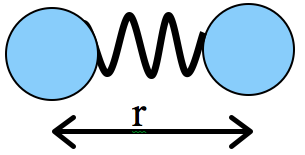
\includegraphics[scale=0.25\linewidth]{act242-massandspring}
\end{center}

Both masses move.  The distance $r$ is the separation of the two masses, measured from their centers.  When they are closer together, the spring is compressed and $r$ is smaller; when they are further apart, the spring is stretched and $r$ is larger.  We let the symbol $r_0$ represent the value of $r$ when the spring is neither stretched nor compressed, i.e., the equilibrium position of the masses.
A)	Make a $PE$ graph of the two-mass \& one spring system.
Let's presume for right now that the spring between the masses acts like an ordinary spring that can compress and stretch:
(1)  On the board, sketch a graph of the $PE$ vs.\ $r$ for the two-mass system described above.  Remember what $r_0$ represents and how an ordinary spring behaves when it is stretched or compressed from its equilibrium position.  Since this is an ordinary spring, don't extend the graph into regions of $r$ that are not physically possible.
(2)  Check to make sure that the force as derived from the $PE$ curve is predicted correctly.
(a)	At $r$ = $r_0$, what is the magnitude and direction of the force (i) based on your experience with springs, and (ii) according to the graph of PE? 
(b)	At $r$ > $r_0$, what is the magnitude and direction of the force (i) based on your experience with springs, and (ii) according to the graph of PE? 
(c)	At $r$ \textless  $r_0$, what is the magnitude and direction of the force i) based on your experience with springs, and (ii) according to the graph of $PE$?
 
\WCD

B)	Now the spring becomes a little ``weird''
(1)	Imagine that the spring becomes much stronger as the masses get closer - so strong that they can never actually touch.  
Make a new graph on the same axes (don't erase your first graph) of the $PE$ of this new system and be prepared to explain how the shape of the $PE$ curve explains the new weird feature.
(2)	More weirdness:  Now in addition to what you did in (1), assume the spring becomes weaker and weaker as the masses move beyond about $2r_0$.  Then, as $r$ continues to increase, the spring becomes so weak that it has hardly any effect even though the masses are still attached.  The spring is just very, very weak.  
Make a totally new second graph of $PE$ below the first graph that shows both of these new behaviors.  Make sure everyone can use the $PE$ curve to explain both of the new weird features of this two-mass system.

\WCD

C)	Making the Graph of the two-mass spring system more useful
Make another  plot of the double weird system on top of the previous graph, but make the spring constant go to zero at a value of the $PE$ that is about twice the previous value.  
Question:  You have just made two graphs with the bottoms of the ``wells'' at the zero of $PE$.  This makes the $PE$ of the two masses for the two springs different when the masses are far apart.  Where could you set the zero of $PE$, so that the $PE$ of both spring systems had the same value when the mass are far apart?  Come to a group consensus and make this combined plot.

\WCD